\documentclass{emulateapj}
\submitted{{\it Submitted for publication in ApJ}}
\usepackage{multirow,color,wrapfig,ulem}
\usepackage {graphicx}
\usepackage{graphics}
\usepackage[dvips]{epsfig}

%=========================================================================
%		INTERNAL MACROS
%=========================================================================
\def\be{\begin{equation}}
\def\ee{\end{equation}}
\def\ba{\begin{eqnarray}}
\def\ea{\end{eqnarray}}

% To highlight comments 
\definecolor{red}{rgb}{1,0.0,0.0}
\newcommand{\red}{\color{red}}
\definecolor{darkgreen}{rgb}{0.0,0.5,0.0}
\newcommand{\SRK}[1]{\textcolor{darkgreen}{\bf SRK: \textit{#1}}}
\newcommand{\SRKED}[1]{\textcolor{darkgreen}{\bf #1}}
\newcommand{\before}[1]{\textcolor{red}{ #1}}
\newcommand{\after}[1]{\textcolor{darkgreen}{ #1}}

\newcommand{\LCDM}{$\Lambda$CDM~}
\newcommand{\beq}{\begin{eqnarray}}  
\newcommand{\eeq}{\end{eqnarray}}  
\newcommand{\zz}{$z\sim 3$} 
\newcommand{\avg}[1]{\langle{#1}\rangle}  
\newcommand{\ly}{{\ifmmode{{\rm Ly}\alpha}\else{Ly$\alpha$}\fi}}
\newcommand{\hMpc}{{\ifmmode{h^{-1}{\rm Mpc}}\else{$h^{-1}$Mpc}\fi}}  
\newcommand{\hGpc}{{\ifmmode{h^{-1}{\rm Gpc}}\else{$h^{-1}$Gpc}\fi}}  
\newcommand{\hmpc}{{\ifmmode{h^{-1}{\rm Mpc}}\else{$h^{-1}$Mpc}\fi}}  
\newcommand{\hkpc}{{\ifmmode{h^{-1}{\rm kpc}}\else{$h^{-1}$kpc}\fi}}  
\newcommand{\hMsun}{{\ifmmode{h^{-1}{\rm {M_{\odot}}}}\else{$h^{-1}{\rm{M_{\odot}}}$}\fi}}  
\newcommand{\Mmin}{{\ifmmode{{M_{\rm min}}}\else{${M_{\rm min}}$}\fi}}
\newcommand{\mmin}{{\ifmmode{{M_{\rm min}}}\else{${M_{\rm min}}$}\fi}}
\newcommand{\mmax}{{\ifmmode{{M_{\rm max}}}\else{${M_{\rm max}}$}\fi}}
\newcommand{\lmmin}{{\ifmmode{{\log M_{\rm min}}}\else{${\log M_{\rm min}}$}\fi}}
\newcommand{\lmmax}{{\ifmmode{{\log M_{\rm max}}}\else{${\log M_{\rm max}}$}\fi}}

\newcommand{\Mmax}{{\ifmmode{{M_{\rm max}}}\else{${M_{\rm max}}$}\fi}}
\newcommand{\dm}{{\ifmmode{{\Delta M}}\else{$\Delta M$}\fi}}
\newcommand{\dlm}{{\ifmmode{{\Delta \log M}}\else{$\Delta \log M$}\fi}}
\newcommand{\focc}{{\ifmmode{{f_{\rm occ}}}\else{${f_{\rm occ}}$}\fi}}

\newcommand{\Msun}{{\ifmmode{{\rm {M_{\odot}}}}\else{${\rm{M_{\odot}}}$}\fi}}  
\newcommand{\msun}{{\ifmmode{{\rm {M_{\odot}}}}\else{${\rm{M_{\odot}}}$}\fi}}  
\newcommand{\lya}{{Lyman$\alpha$~}}
\newcommand{\clara}{{\texttt{CLARA}}~}
\newcommand{\rand}{{\ifmmode{{\mathcal{R}}}\else{${\mathcal{R}}$ }\fi}}  
%SAMPLES


%MY COMMANDS #############################################################
\newcommand{\sub}[1]{\mbox{\scriptsize{#1}}}
\newcommand{\dtot}[2]{ \frac{ d #1 }{d #2} }
\newcommand{\dpar}[2]{ \frac{ \partial #1 }{\partial #2} }
\newcommand{\pr}[1]{ \left( #1 \right) }
\newcommand{\corc}[1]{ \left[ #1 \right] }
\newcommand{\lla}[1]{ \left\{ #1 \right\} }
\newcommand{\bds}[1]{\boldsymbol{ #1 }}
\newcommand{\oiint}{\displaystyle\bigcirc\!\!\!\!\!\!\!\!\int\!\!\!\!\!\int}
\newcommand{\mathsize}[2]{\mbox{\fontsize{#1}{#1}\selectfont $#2$}}
\newcommand{\eq}[2]{\begin{equation} \label{eq:#1} #2 \end{equation}}
\newcommand{\lth}{$\lambda_{th}$ }
\newcommand{\reff}{{\ifmmode{r_{\mbox{\tiny eff}}}\else{$r_{\mbox{\tiny eff}}$}\fi}}
%#########################################################################

%TO DO COMMANDS. Highlight region that needs extra work  #############################################################
\newcommand{\todo}{\ifmmode \text{\Huge{\(\bullet\)}} \else {\Huge$\bullet$}\fi}
% \newcommand{\todo}{\ifmmode {\Huge \bullet} \else {\Huge$\bullet$}\fi}
\newcommand{\tido}{\ifmmode {\bullet} \else $\bullet$\fi}
\newcommand{\REFS}{(\todo REFS) }
\newcommand{\toref}{(\todo REFS)}
%#########################################################################



\begin{document}
%=========================================================================
%		FRONT MATTER
%=========================================================================
\title{The Spatial Distribution of Local Group Satellites in a
  Cosmological Context}  
\author{
  Ver\'onica Arias \thanks{v.arias@uniandes.edu.co}$^{1}$,
  Jaime E. Forero-Romero \thanks{je.forero@uniandes.edu.co}$^{2}$ 
}

\affil{
$^1$Departamento de F\'{i}sica, Universidad de los Andes, Cra. 1
No. 18A-10, Edificio Ip, Bogot\'a, Colombia\\
}

\begin{abstract}
We focus on the spatial distribution of bright ($M_V<-8$) satellites and
pairs of galaxies with similar masses, isolation and kinematic
configurations as the Local Group. 
\end{abstract}

\keywords{
Galaxies: halos --- Galaxies: high-redshift --- Galaxies: statistics
--- Dark Matter --- Methods: numerical 
}

\section{Introduction}

Since the early works of (el que libeskind dice que habló de
eso primero) and \cite{1976MNRAS.174..695L}, the observed anisotropic
distribution of satellite galaxies in the Local Group has been a key
point in the discussion of galaxy formation models within $\Lambda$CDM
cosmology. These pioneer papers described that the then known satellite
galaxies of the Milky May (MW) were distributed roughly following the plane
that contained the Magelanic clouds and their stellar tails. This
anisotropic distribution was further studied in the work of \cite{}Pawlowski
et. al. (2012), where they included all the known MW satellite galaxies (XXX
more than in the original Lynden-Bell paper) as well as some MW globular
clusters, and found that they are all contained in what they call a
"Vast Plane Of Satellites" (VPOS). This structure is around 30kpc thick and
is perpendicular to the stellar disc of the MW galaxy. This plane of
satellites was considered a rarity until the PAndAS survey of the
Andromeda (M31) galaxy and its halo (missing reference on the survey)
provided a complete sample of the satellite galaxy population (above a
XXXX magnitude) of our neighboring galaxy, allowing their consistent distance
estimations (Conn et al. 2012). In a groundbreaking work, Ibata et
al. (2013) found that 15 out of the 30 satellites are in a planar
structure that is 15kpc thick and has an extension of 400kpc.
Additionally, from line of sight velocity measurements, they
found that the structure has an apparent coherent rotation, with the
satellites south of M31 moving away from us and those north of M31
coming towards us. This apparent organized rotation of satellite galaxies was also
statistically found to occur in diametrically opposed 
pairs of satellites from the SDSS (Ibata et al. 2014), although this
results were contested in a follow up paper by Cuatun et al. (2014).  

These discoveries of the planes in M31 and the MW were followed by the
remark from Shaya et al. (2013) that the other satellite galaxies in
M31 could be part of a second plane, further reinforcing the idea that
satellites in the local group are not isotropically distributed.
Despite the challenges in estimating distances to the satellites
galaxies, Tully et al. managed to go beyond the local group and found
two planes of satellites galaxies in Centaurus A, making a clearer
case for the planes of satellites: in all the galaxies where distance
measurements could be performed evidence of satellite planar
structures have been found.\\

These observed planes and their apparent co-rotation seem to challenge
current galaxy formation models (Pawlowski et al. 2014).
\cite{2012MNRAS.424...80P} compared the kinematic structure of the MW
satellites against DM only simulation of high resolution halos from
the Via Lactea and Aquarius projects and could not find find a similar
kinematic structure (i.e. the orbital poles of the MW satellites) in
the simulations. Additionally, a few months after the discovery of the
M31 plane of satellites, Bahl and Baumgardt (2013) looked for similar
structures in the MilleniummII dark matter only cosmological
simulations, and found that planar structures are common (they found
them in around 2 per cent of host halos). Nevertheless these results
were contradicted by the works of Ibata el al. (2014) and Pawlowski et
al. (2014) who, analyzing the same cosmological simulations with
methods closer to those used to analyze the observational data, found
that planar structures such as that observed in M31 are extremely rare
(less than 0.02 per cent or 0.004 per cent respectively). But
satellite galaxies are not particularly good tracers of the underlying
dark matter structure (Sawala 2014), and indeed anisotropic
distributions of the satellites have been found in the APOSTOLE
simulations that include baryonic physics \citep{2016MNRAS.457.1931S},
although the Milky Way remains an extreme case. These results were
contested by \cite{2015ApJ...815...19P} who claim that the
anisotropies found are a product of using a metric that ignores the
radial position of the galaxies. %Sawalla et al. 2014
In CLUES, a high resolution constrained Local Group simulation,
Gillet et al. (2015) found M31-like planes but again, the observed M31 plane
remains an extreme case, and this seems to be corroborated by Cautun
et al. (2015), who, despite finding a great variety of planes in
simulations remarks that the observed M31 plane has an "unusually large
radial extent".\\  

In addition to these plane-finding efforts in cosmological simulations,
many works have focused on the possible formation processes that led
to planar structures and on the alignments  of these structures with
the cosmic web. In a pioneer work \cite{2011MNRAS.411.1525L} measured
the infall direction of satellites in a DM only constrained simulation of one pair
of LG halos and found that there is a definite infall direction. 
% but it's not quantified in terms of the cosmic web.
Using cosmological dark matter only simulations
\cite{2014MNRAS.443.1274L} showed that the preferential infall
direction was along cosmic filaments, result that was also obtained by 
\cite{2015ApJ...799..212L}. This result was further
confirmed by \cite{2015MNRAS.450.2727T}, who measure the angle between
satellites and the direction defined by filaments (Bissous filament
finder) to find a signal both in the SDSS galaxy catalog and in the
semi-analytic galaxies in the Millennium Simulation. Additionally, 
an analysis of the cosmic flow data set by Libeskind et al. (2015) 
reveals that four out of the fives satellite planes observed in the 
Local Group are aligned with a filament. 
Additionally, \cite{2016arXiv160601516L} use the SDSS DR10 catalog to study galaxy pairs and find that satellites tend to accumulate towards the companion galaxy: There
are up to $\sim 10\%$ more satellites in the space between the pair
than expected from an uniform distribution. 

Early filamentary accretion has been proposed as the formation mechanism for the Andromeda thin plane of satellites (Buck et al 2015), with early formed galaxies accreting their mass via cold thin filaments. 
This formation mechanism results naturally in thin planes, but a follow up work shows that these are not kinematically coherent structures (Buck et al. 2015). These results are from dark matter only simulations, so it would be interesting to see if they still hold for simulations that include baryonic physics, since it was shown by Gonzales et al 2015 that satellites acrreted via filaments are destroyed faster than those that are not. 

In a more general numerical study,   
\cite{2016arXiv160501728S} use the eagle simulation to study the
alignment of satellites with respect to the central galaxy. They find
a weak alignment. Around $20\%$ of the systems have a misalignment
angle larger than the value observed for the Milky Way. 


Planes in simulations tend to be transient structures (not
kinematically coherent) and that poses two problems: one is why do we
see planes in all the galaxies were we can actually make the
measurements if they are transient? Problem with the MW plane for which
some of the dwarfs have proper motion measurements. Another problem:
explicación de Buck 2015 sería rara entonces...


\section{Numerical Setup}

\subsection{Illustris simulation}

In this work we use the publicly available results from the Illustris
simulation (Vogelsberger et al. 2014). This cosmological simulation, performed using
the quasi-Lagrangian code AREPO, follows the coupled evolution of dark
matter and gas, and includes parametrizations to account for the effects of
gas cooling, photoionization, star formation, stellar feedback, black
hole and super massive black hole feedback. Vogelsberger et al. 2014 use a $75 Mpc/h$
simulation box, with $\Lambda$CDM cosmology initial conditions
starting at a redshift $z=127$ and consistent with WMAP-9 measurments.

\subsection{Sample Selection}

We select all halos with maximum circular velocities in the
range 150 km s$^{-1}$ $<V_{\rm max}<$ 350 km s$^{1}$.
We exclude sub-halos from this selection.
From this set we construct a sample of pairs as follows.
For each halo $A$ we find its closest halo $B$, if halo $A$ is also
the closest to halo $B$, the two halos are considered as a pair. 
Another way to phrase this selection is that pairs do not have
neighbors closer than the pair's distance.
We exclude the pairs that are closer than
There are $53$ pairs with those conditions in the simulation.

We extract from the simulation spheres of $2$ \hMpc  in radius around
the pair's center of mass. 
We use this information to exclude all the pairs that have separations
smaller than the sum  of their virial radii, i.e. we exclude
interacting pairs. 
This reduces to $49$ the number of pairs in the sample.

We count the number of galaxies with $M_V<-9$ inside the virial
radius of each halo, including the central galaxy.
We only keep pairs where both halos have 5 bright galaxies at least. 
This reduces the sample to $24$ pairs. 
We call this sample the Full Sample.

From the Full Sample we build a second sample based on the pairs' kinematics. 
Figure \ref{fig:samples} shows the co-moving separation and relative
speed between the two halos in the pair.
The stars in the Figure represent the pairs with a separation in the
range $0.75\hMpc <R_{AB}< 1.50\hMpc$ and relative velocity in the
range $V_{AB}>100$ km s$^{-1}$, which are close to the Local Group
Observed values.
We call this sample the LG Sample.

The number of pairs in the Full Sample is consistent with previous
calculations. 
\cite{ForeroRomero2013} performed a study of the LG kinematics using a
cosmological N-body simulation as a benchmark. 
In their study, using criteria similar to ours to define the Full
Sample, they found 1923 pairs in a volume of $250^3$ $h^{-3}$
Mpc$^{3}$. 
With the same number density we expect to find $52$ pairs in the
volume of the Illustris simulation, which is very close to the actual
number of $49$ pairs.

In the same study they found 158 pairs with broad kinematic
characteristics, similar to the definition of our LG sample. 
This represents a reduction of a factor of $12$ from their General
Sample. 
With those numbers in mind we would expect to keep at least $4$ pairs
in the Illustris volume. 
Given that our conditions are slightly more relaxed (we do not ask for
isolation criteria from massive halos) we end up with a larger sample
size, but still consistent with the fact that LG-like pairs are
scarce.  
%no me es muy claro este ultimo parrafo. En nuestros samples pasamos de 49 a 24 (o sea se redujo en un factor 2 en vez de un factor 12)

\begin{figure}
\centering
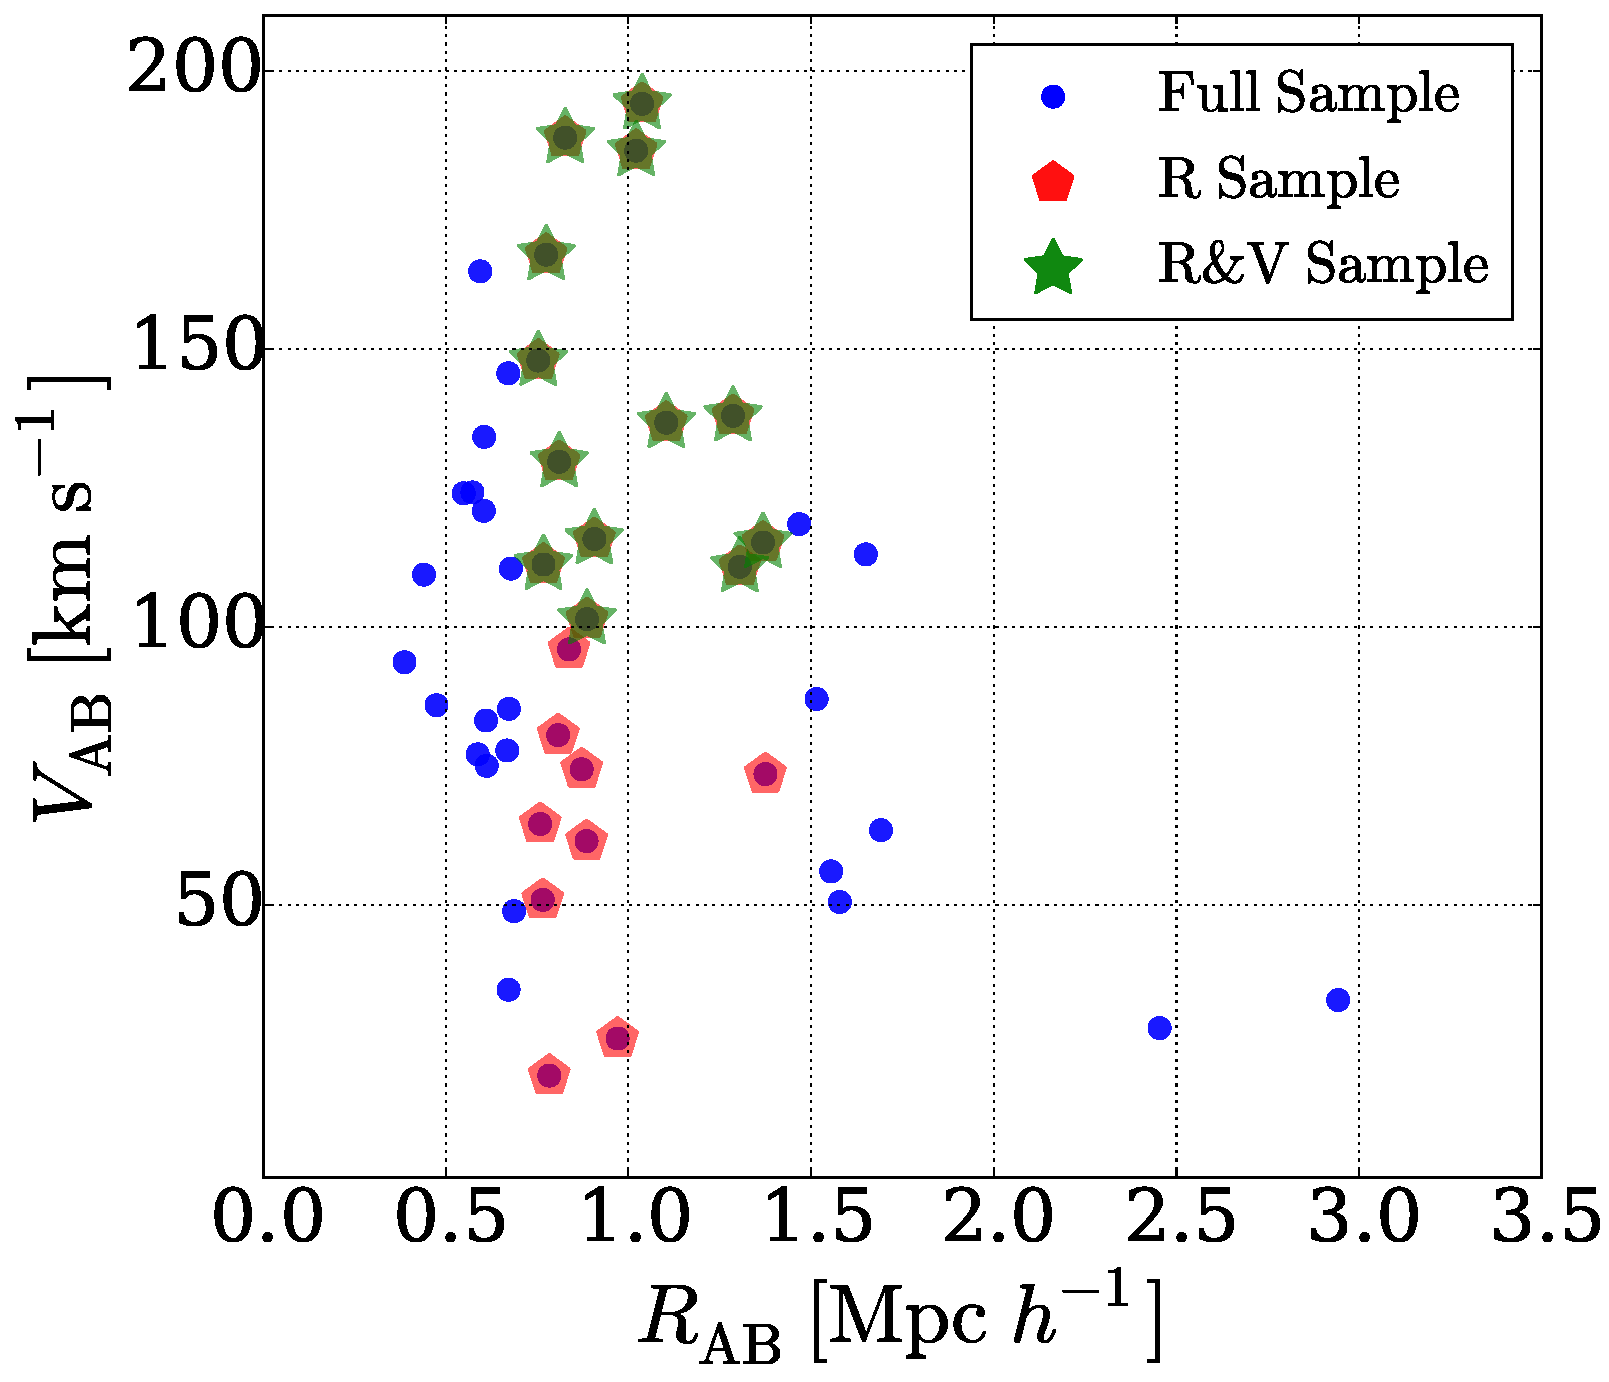
\includegraphics[width=\hsize]{v_r_pairs.pdf}\\
\caption{Halo pair samples used in this paper located in the
  plane of relative comoving velocity $V_{AB}$ versus relative
  distance $R_{AB}$ between the two halos in the pair.
  The R\&V sample is the closest to the separation and kinematic
  conditions observed in the Local Group.} 
\label{fig:samples}
\end{figure}

%\begin{figure}
%\centering
%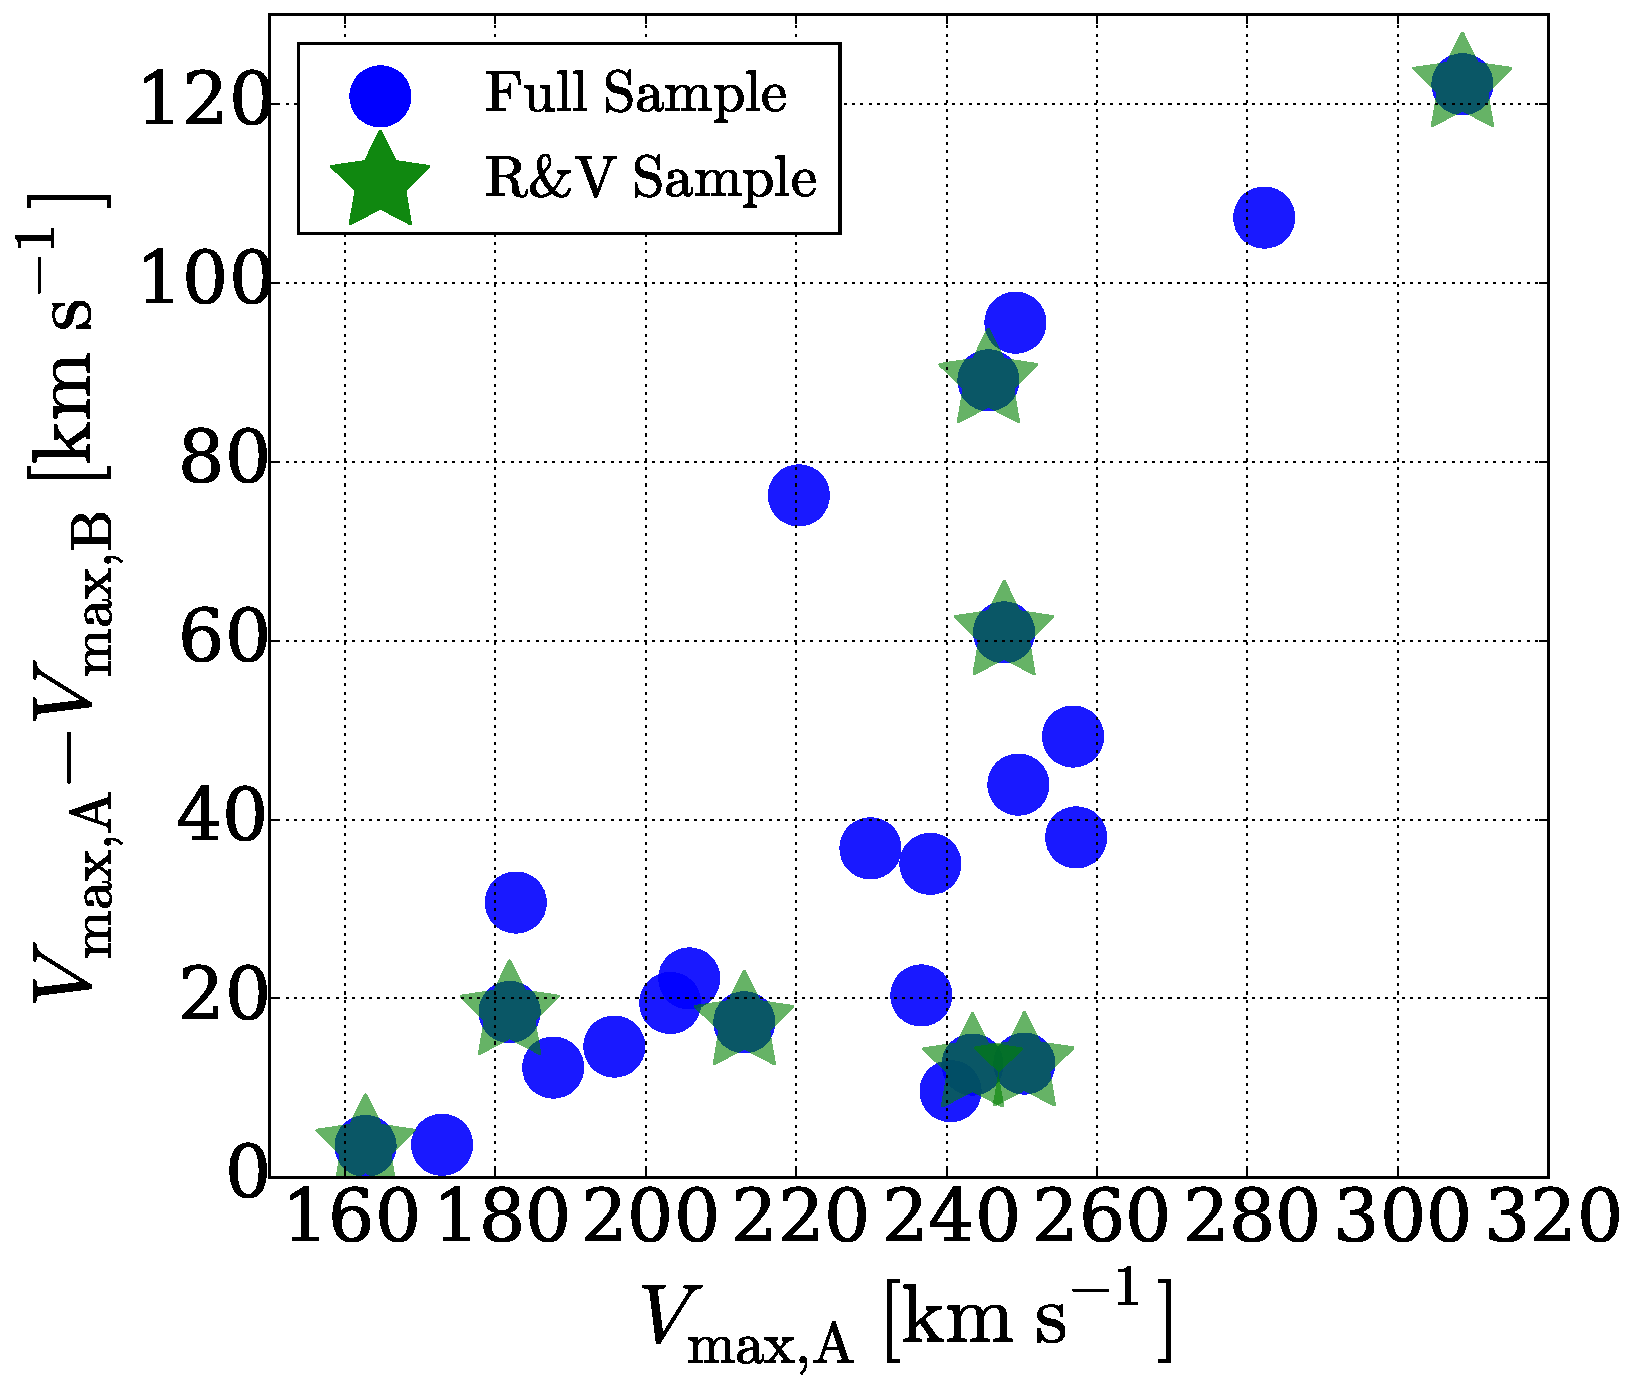
\includegraphics[width=\hsize]{v_circ_pairs.pdf}\\
%\caption{Diference between the maximum circular velocity $V_{max}$ for the two
%  halos in the pair as a function of $V_{max}$ for the massive halo in
%  the pair.}
%\label{fig:vcirc}
%\end{figure}

\begin{figure}
\centering
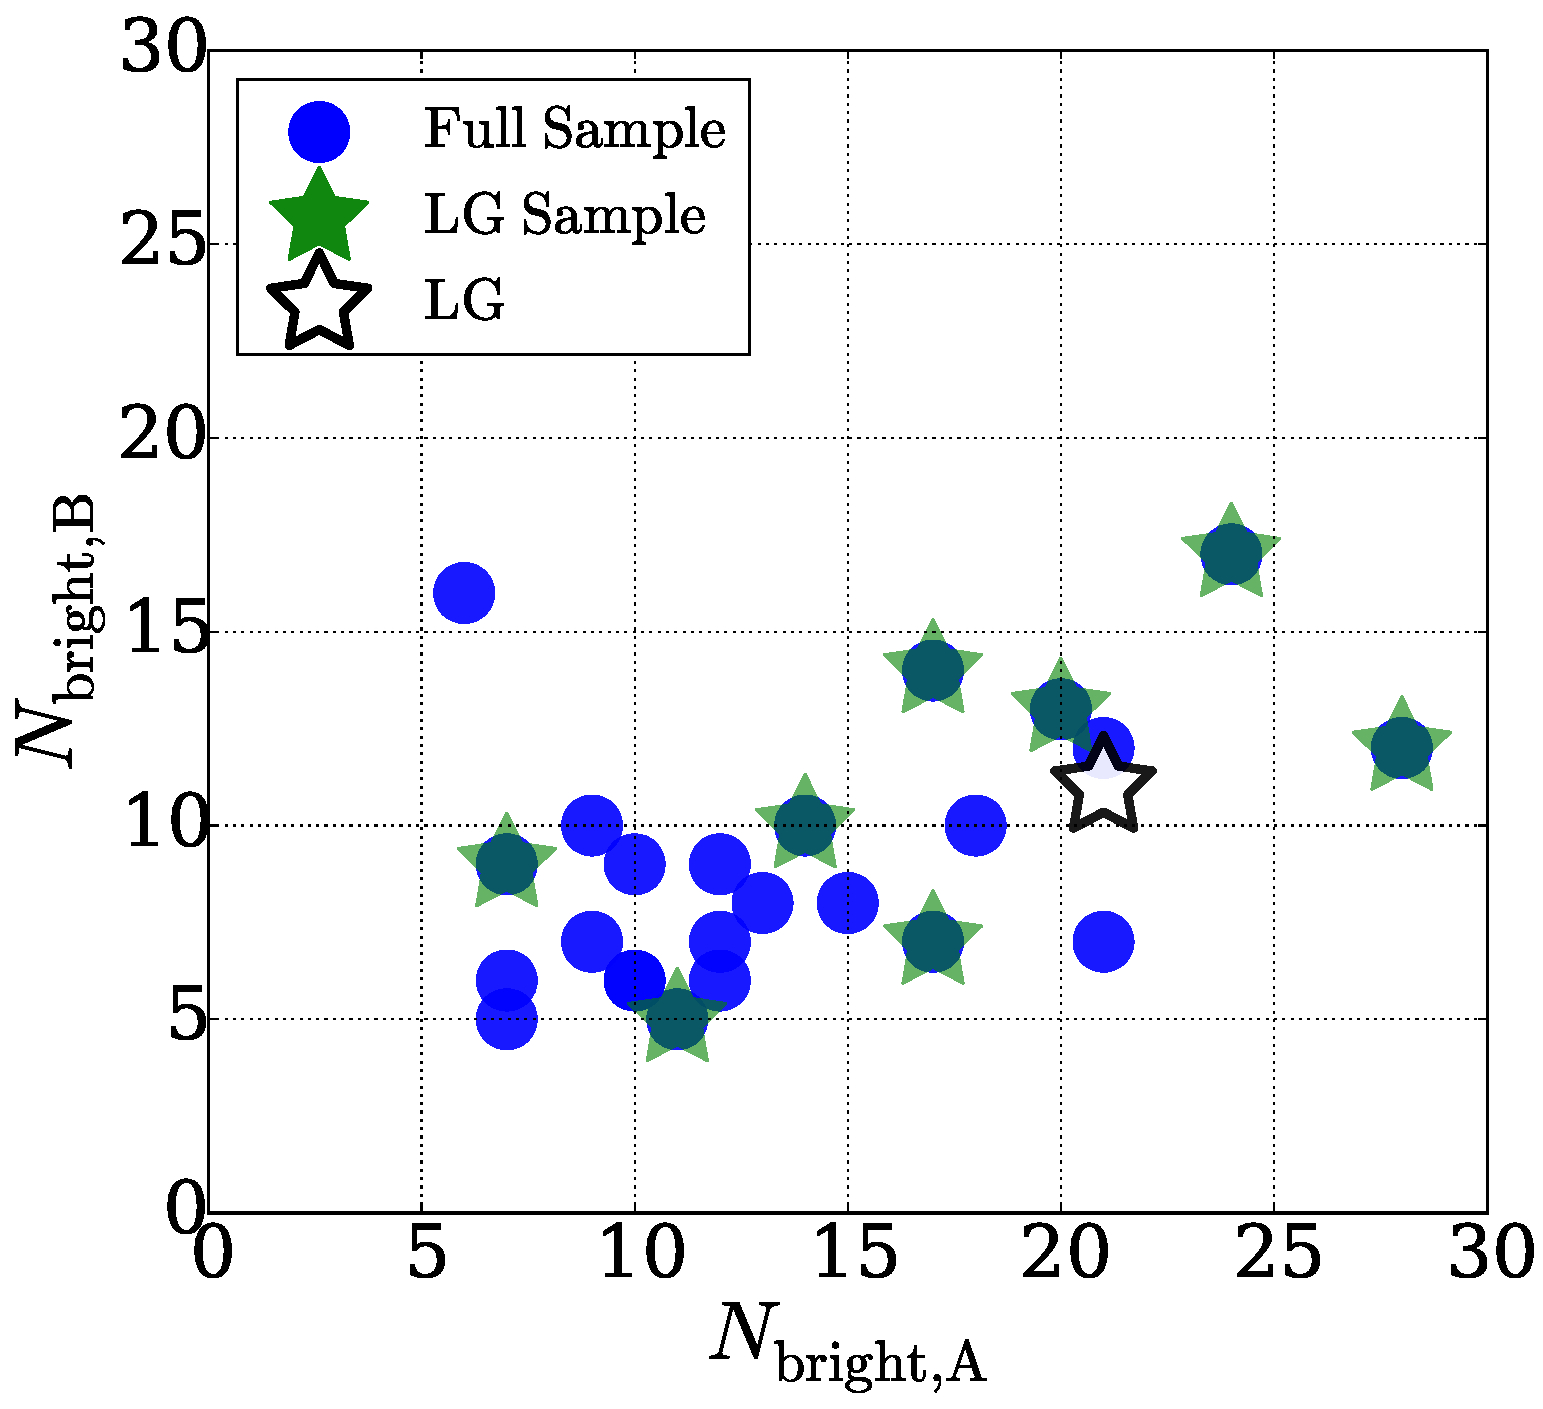
\includegraphics[width=\hsize]{n_structure.pdf}\\
\caption{Number of bright substructures ($M_{B}<-9$) and dark matter
  substructures.}
\label{fig:nstructure}
\end{figure}


\subsection{Cosmic Web environment}
%me parece que la palabra "place" puede ser confusa. 
We place the pairs in our sample into the cosmic web as quantified by
the deformation tensor.
\citep{2007MNRAS.375..489H,2009MNRAS.396.1815F}.
This method computes a cartesian grid the tensor $T_{ij}$,
\begin{equation}
T_{ij} \equiv \frac{\partial^2\phi}{\partial r_i \partial r_j}
\end{equation}
%
where $\phi$ is a pseudo-gravitational potential that follows the
Poisson equation $\nabla^2\phi=-\delta$ and the $r_i$ coordinates
correspond to a cartesian system with $i=1,2,3$. 

This tensor is and symmetric and can be diagonalized.
Its eigenvalues ($\lambda_1 > \lambda_2 > \lambda_3$) and
corresponding eigenvectors ($\hat{e}_1$, $\hat{e}_2$, $\hat{e}_3$)
define the degree and direction of stability around the neighborhood
where the tensor was computed. 
This allows the classification of that region either as a peak,
filaments, sheets and voids in the case of three, two, one or zero
eigenvalues larger than a given threshold $\lambda_{th}$.

In this study we compute these eigenvalues and eigenvectors over the
dark matter component of the Illustris-3 simulation on a cubic mesh of
$74$ cells on a side. 
This resolution corresponds to $\sim 1$ Mpc h.
We interpolate the DM density on that mesh using a Cloud-In-Cell (CIC)
scheme. 
We proceed to smooth the density field with a gaussian window with a
physical scale equal to the cell size. 

We choose this interpolation and smoothing scale for two reasons.
First, because it corresponds to the typical pair separation in our
sample.
Second, because it allows a direct comparison with other results in
the literature that used the same methodology to quantify the cosmic
web environment for Local Group pairs in a cosmological context
\citep{ForeroRomero2013,2015ApJ...799...45F}.  

\subsection{Characterization of spatial distributions}
\label{Method}
In this paper, our aim is to study alignments: of the
satellite population with the cosmic web, of the dark matter halos
with the axis that unites them, etc... To do this, we fitted a triaxial spheroid to both the satellite (bright) and the dark matter (dark) subhalo distributions, to get both their semi-major and semi-minor axis.
With this geometrical information we can study the alignments of the two distributions with the cosmic web, and also with the vector that unites the halo pair that host these substructures. %Jaime, falta el plot de alineaciones con la cosmic web

\section{Results}
\label{Results}

Some papers claim that once baryonic physics is included more planar distributions are found.
First we investigate if there is a difference in the bright and dark distribution in terms of their flatness.
In Figure \ref{fig:StreamPlaneOrbit} we can see that indeed the bright distribution is flatter than the dark distribution.
\begin{figure}
\centering
\includegraphics[width=\hsize]{axratio_dark_bright.pdf}\\
\caption{Axis ratio of luminous satellites versus the axis ratio for
  dark subhalos.}
\label{fig:StreamPlaneOrbit}
\end{figure}

We then try to fit planes to both the dark and bright distributions in order to test if it is indeed easier to find thinner planes in the bright distribution. 
We find that the bright planes are thinner.
\begin{figure}
\centering
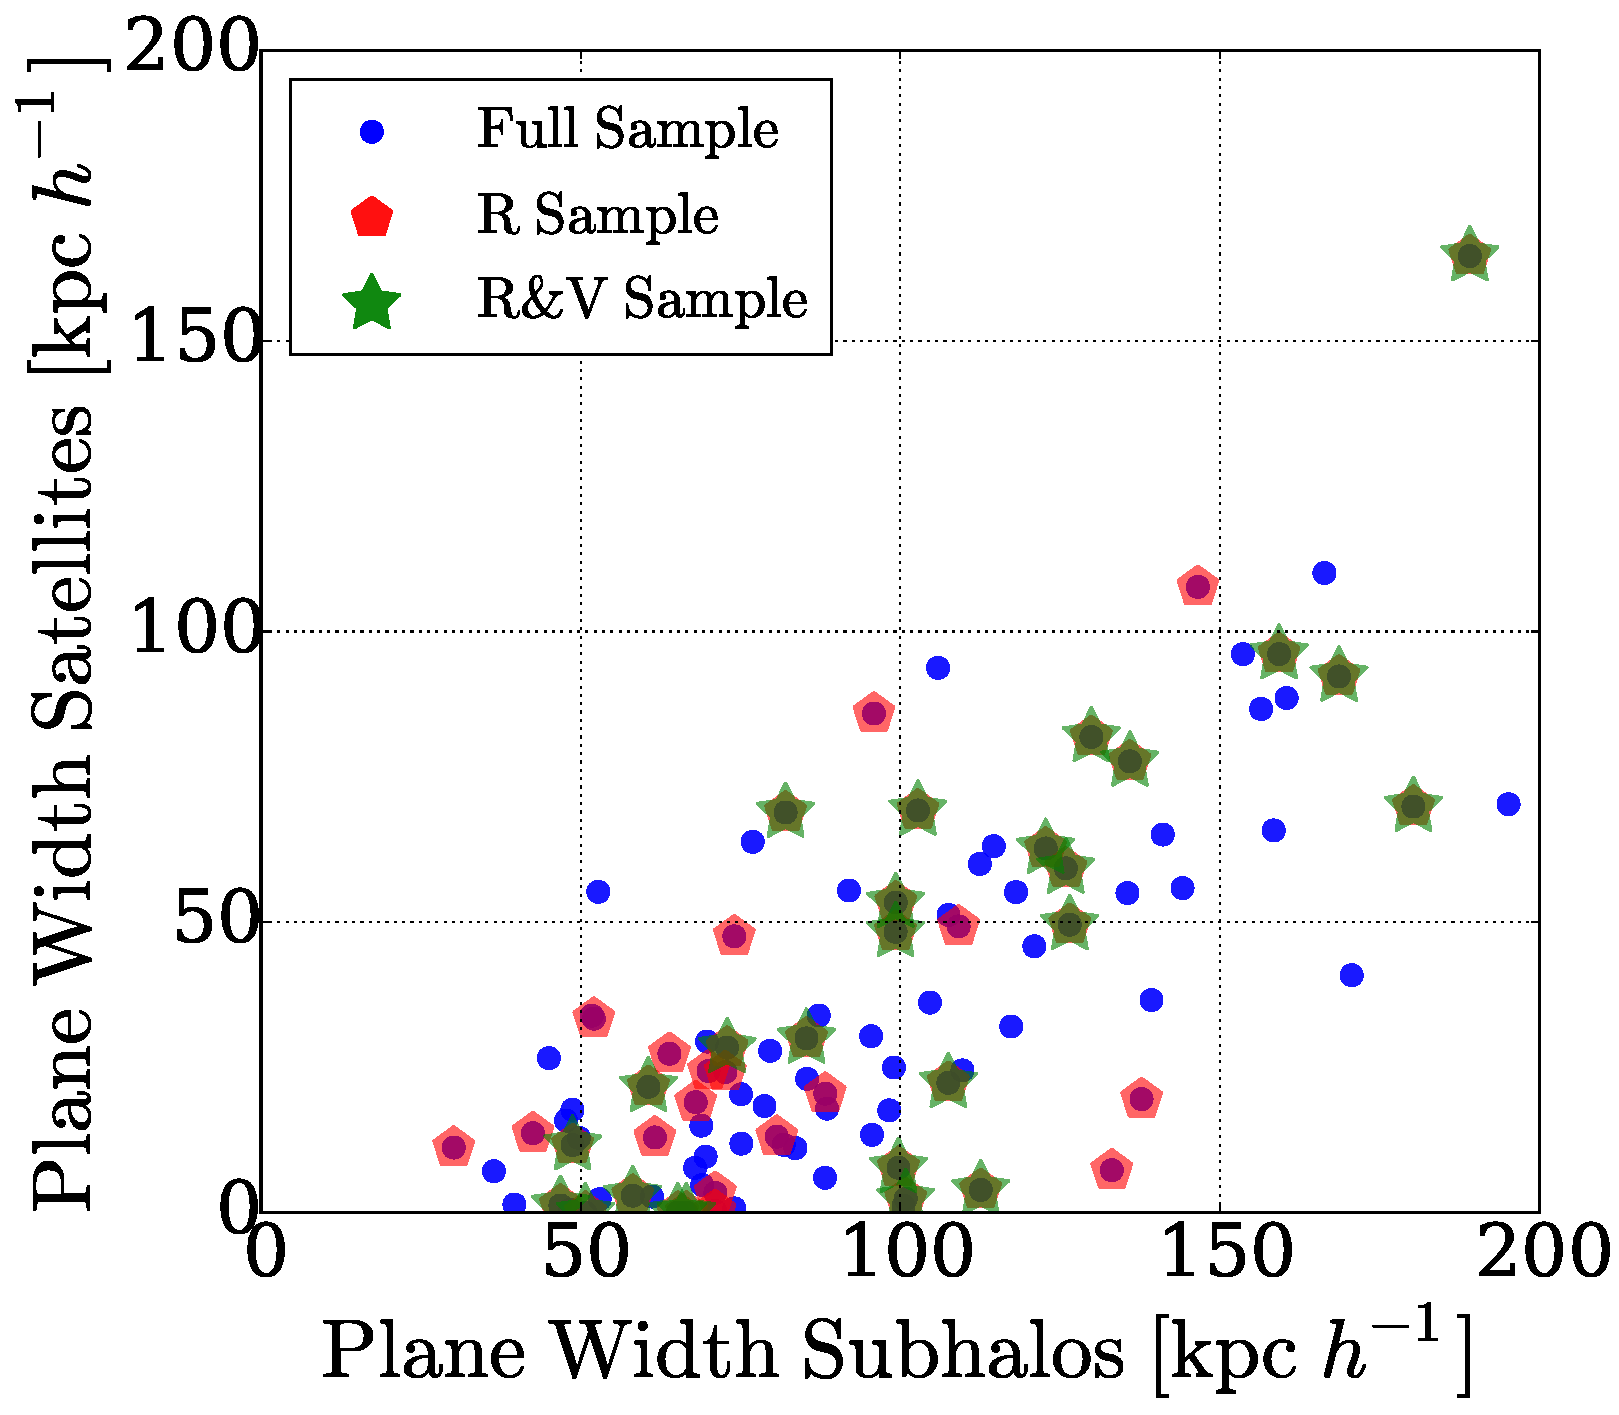
\includegraphics[width=\hsize]{plane_width.pdf}\\
\caption{Plane width for the best planes in the luminious and dark cases.}
\label{fig:plane_width}
\end{figure}
But is there a physical reason for that? Apparently not, since the thinness of the fitted planes seems to be only due to number of objects: number of bright satellites is smaller than of dark sub-halos and that results naturally in thinner fitted planes.
%pregunta para Jaime: en tu código dark quiere decir dm only subhalos o todos los subhalos (dm only y bright)?
%podríamos hacer como un test extra el plot que yo tenía en mis plot de antes, que es cojer al azar entre los dark un numero de subhalos igual al de bright y ver los anchos de los planos.

\begin{figure}
\centering
\includegraphics[width=\hsize]{plane_width_n_dark.pdf}\\
\caption{Plane width as a function of objects used to find the plane.}
\label{fig:plane_width_nobjects}
\end{figure}

A second test is to look if there is any evidence of alignments between the distribution of satellites and the axis that unites the main halos that form the pair. 


\begin{figure}
\centering
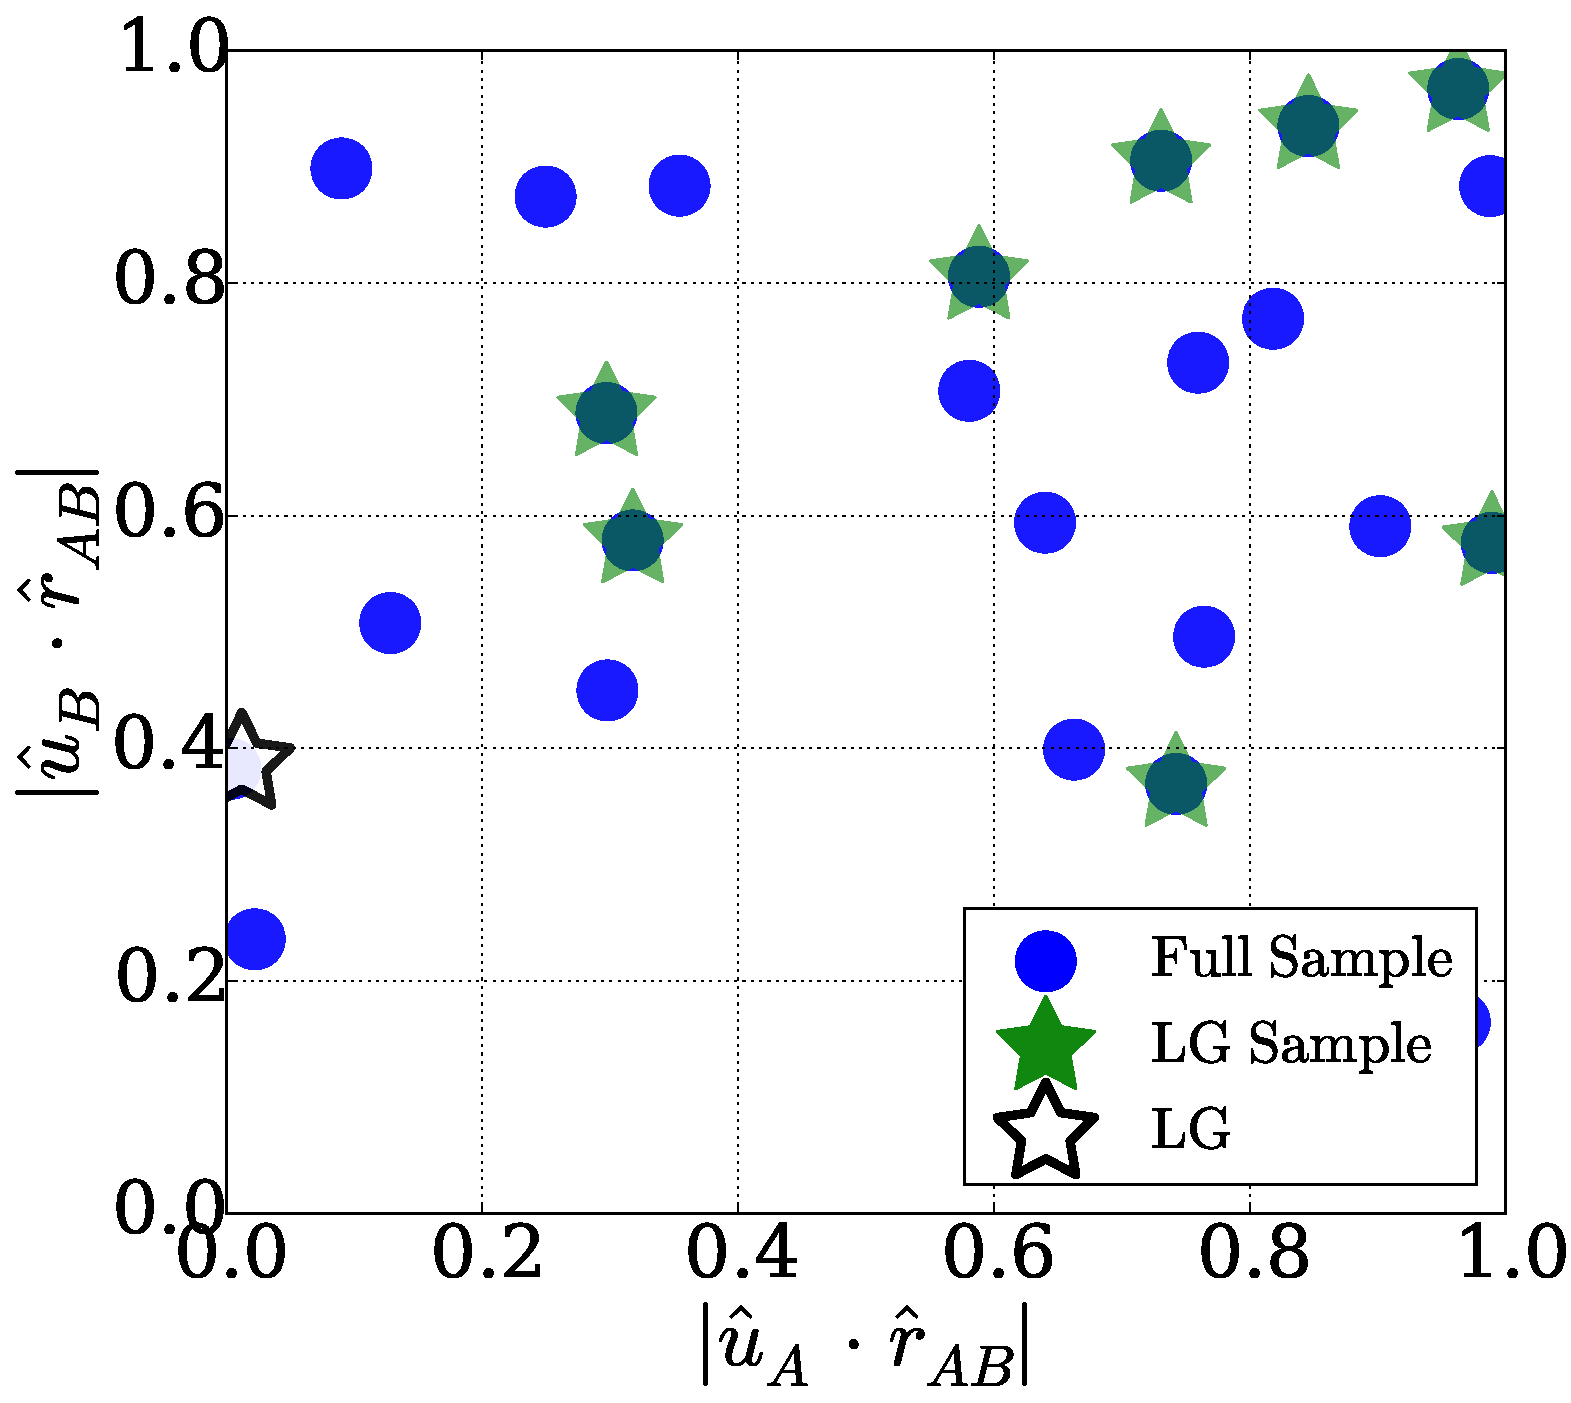
\includegraphics[width=\hsize]{r_u_alignment.pdf}\\
\caption{Alignment of the mayor axis with the vector connecting the
 two halos.}
\label{fig:lg_alignment}
\end{figure}

\begin{figure*}
\centering
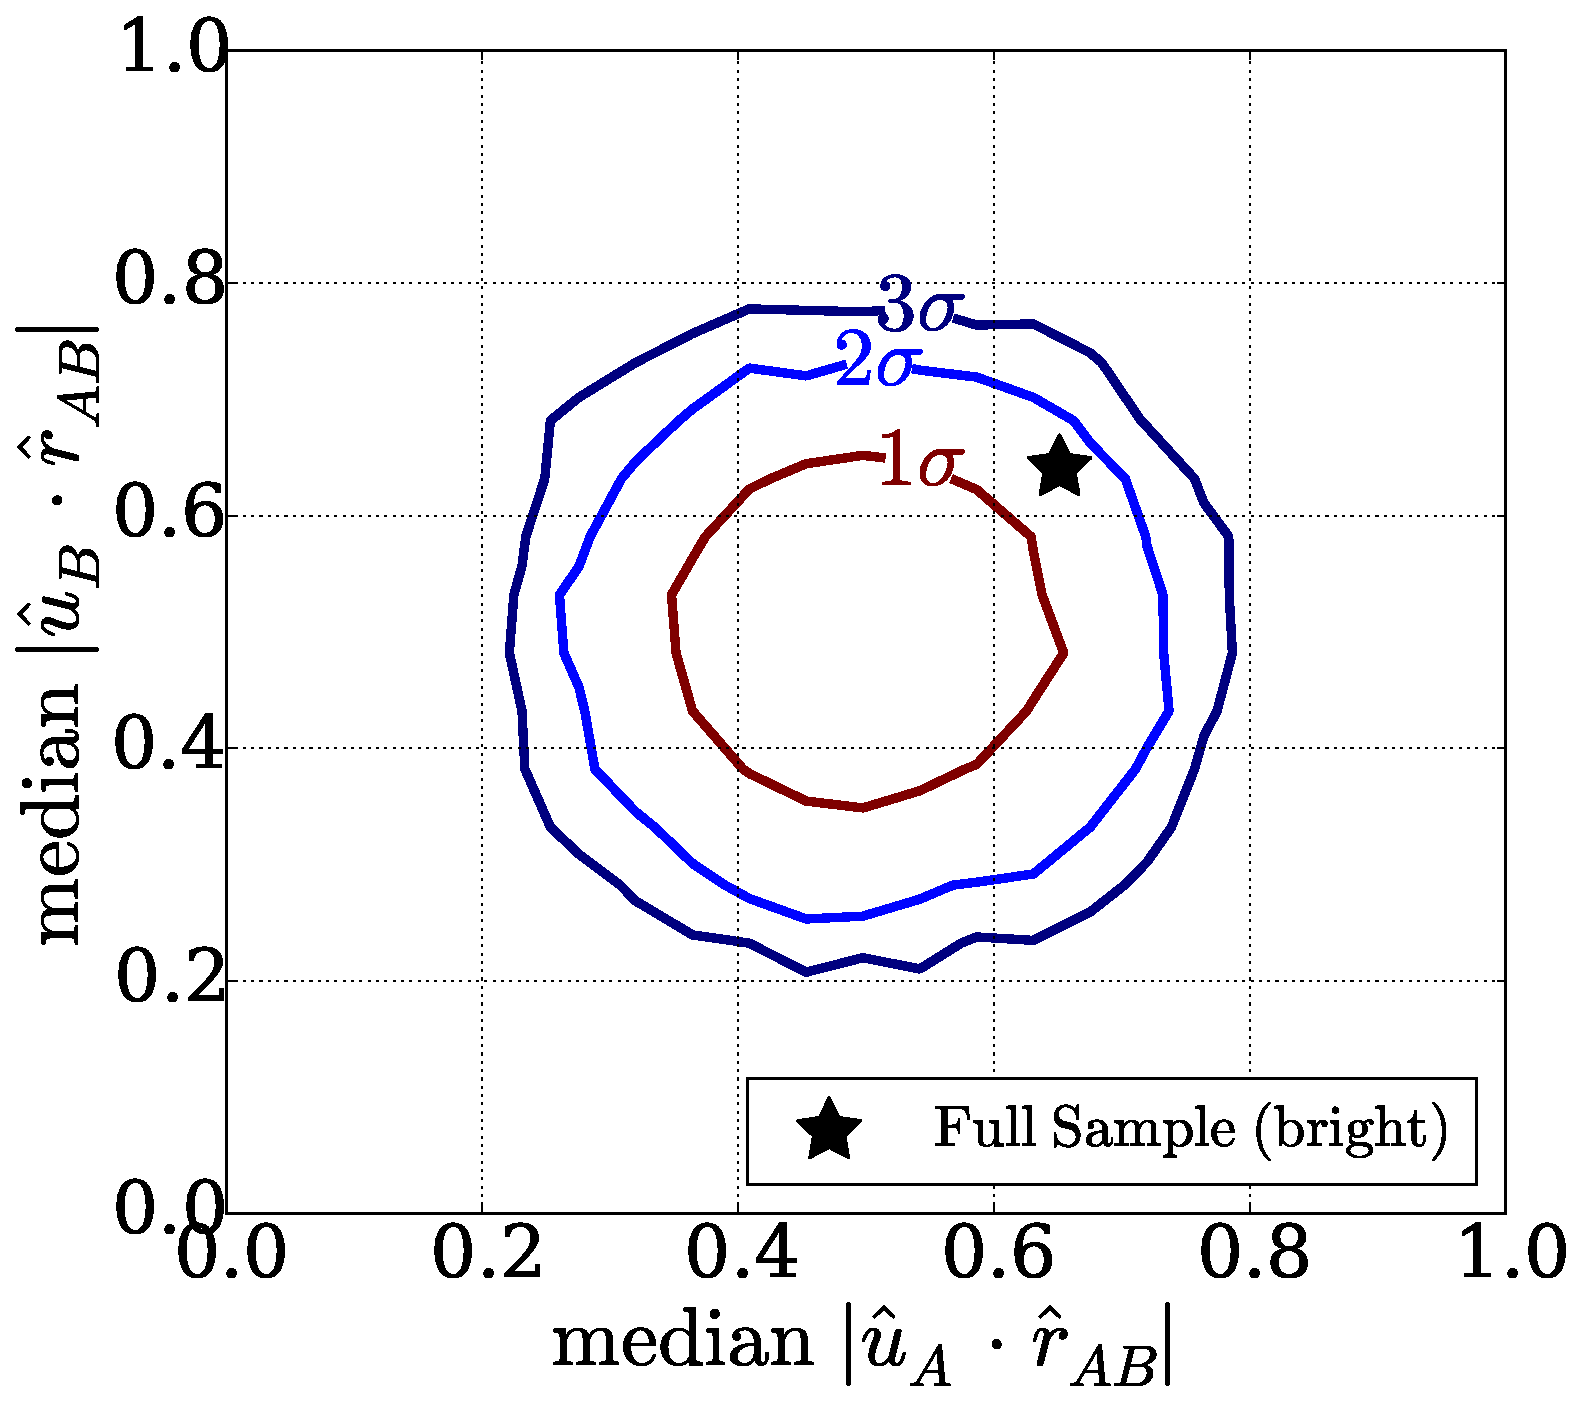
\includegraphics[width=0.48\hsize]{significance_full_bright.pdf}
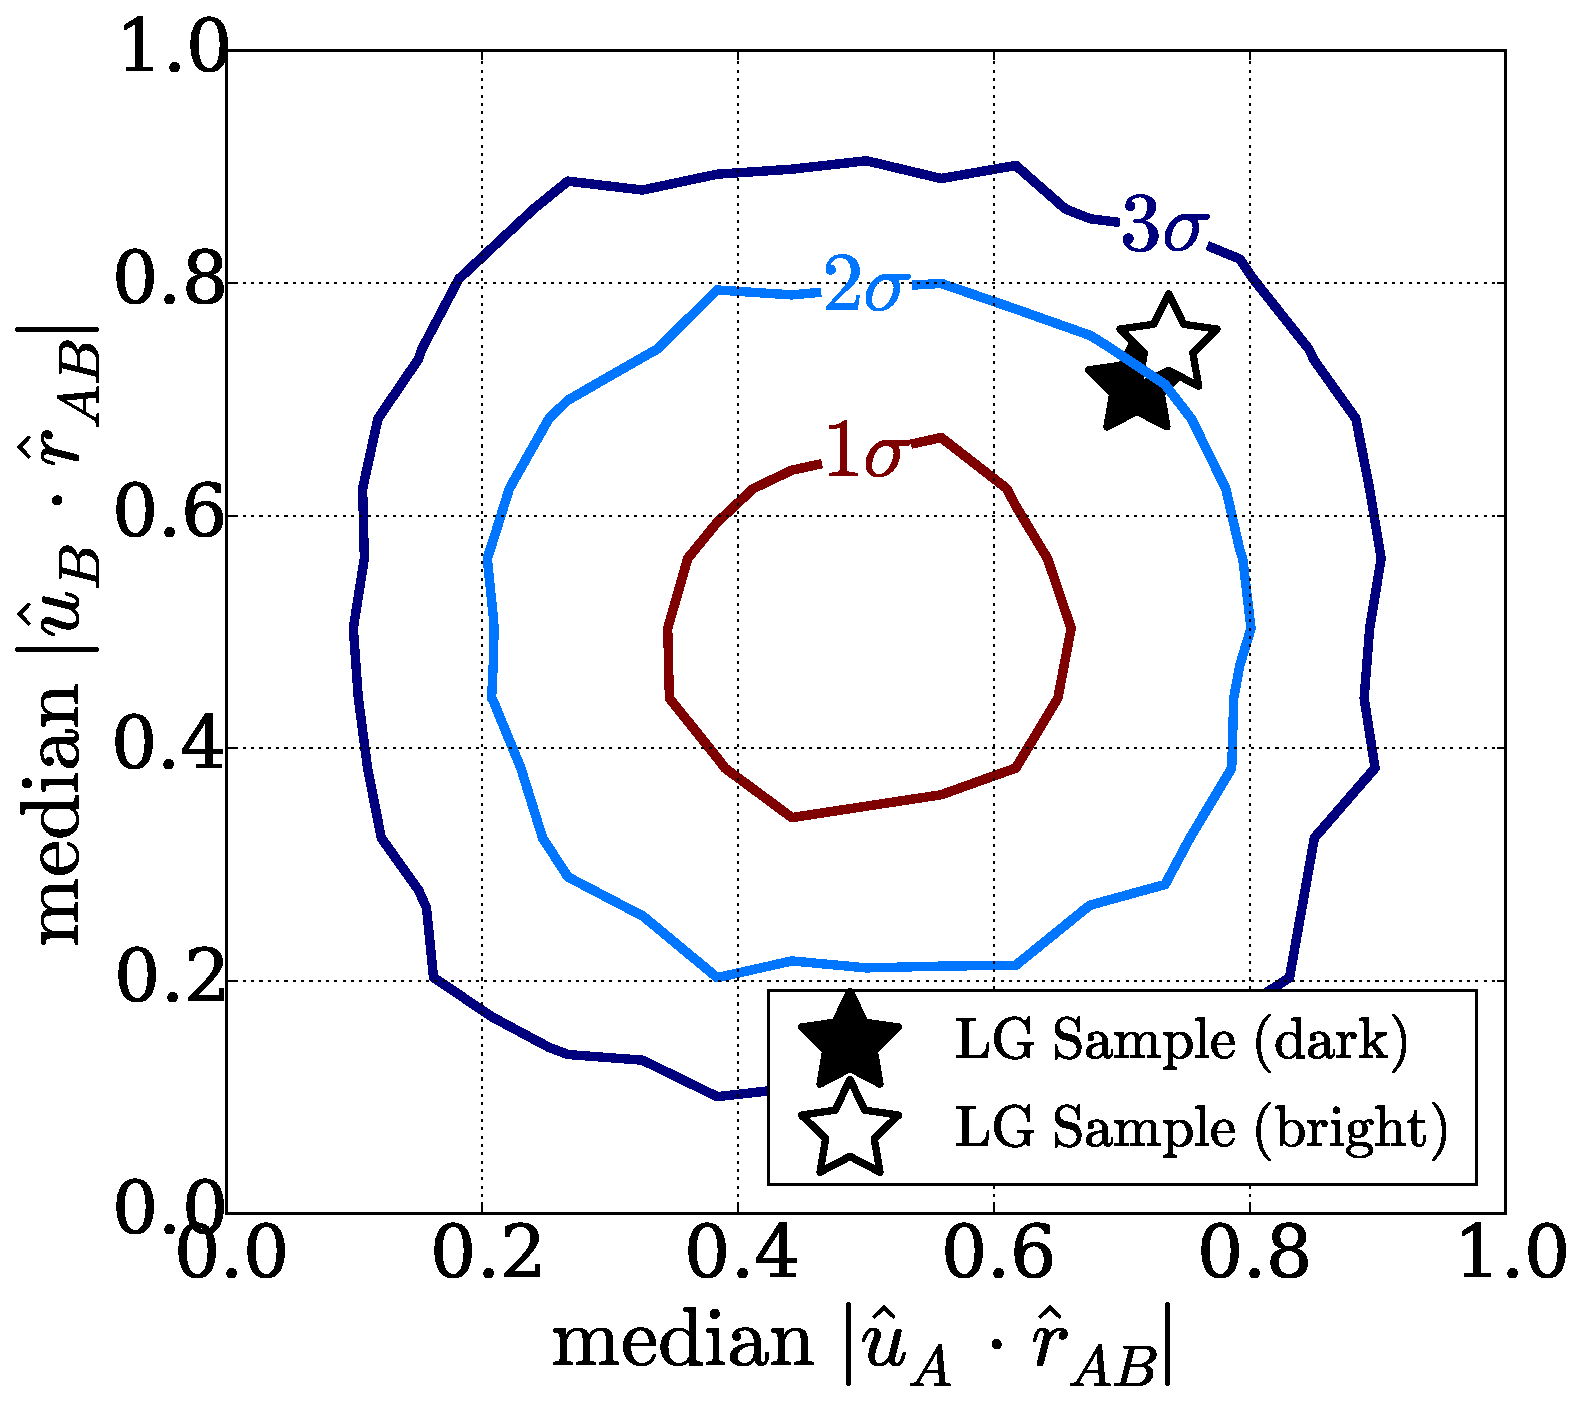
\includegraphics[width=0.48\hsize]{significance_lg_bright.pdf}
\caption{Significance of alignments for both samples.}
\label{fig:significance}
\end{figure*}


%\begin{figure}
%\centering
%\includegraphics[width=\hsize]{Halo_pos_LRomulusRemus.pdf}\\
%\end{figure}

\section{Discussion}
Difference between bright and dark distributions are only due to number.\\
We find significant alignments between distributions and H1H2 axis. But this alignments are the opposite as the one observed for the Local Group!!! 
 
\section{Acknowledgements}
Gracias.

%\begin{wraptable}{l}{2\linewidth}
%\centering
%\begin{tabular}{|l|l|l|l|l|l|}
%\hline
%Bahl 2013       & MilleniumII & resolution & number of host halos& gas no        & planes yes? \\\hline
%Ibata 2014      & MilleniumII & resolution & number of host halos& gas no        & planes no? \\\hline
%Pawlowski 2015  & MilleniumII & resolution & number of host halos& gas no        & planes no? \\\hline
%Gillet 2015     & CLUES       & resolution & number of host halos& gas yes and no& planes yes \\\hline
%Cautun 201XXX   & ?           & resolution & number of host halos& gas ??????    & planes yes \\\hline
%Buck            & their own   & resolution & number of host halos& gas no?       & planes yes \\\hline
%Sawala          & Apostole?   & resolution & number of host halos& gas yes?      & planes yes \\\hline
%Gonzalez        & their own?  & resolution & number of host halos& gas yes/no    & planes he does not care \\\hline
%\end{tabular}
%\end{wraptable}

%Simulation papers:
%%\item {ya}
%%\item{Bahl and Baumgardt 2013 "A comparison of the distribution (...)":\\
%%MilleniumII and a semi-analytic model\\
%%Baryonic mass cut: 2.8$\times 10^4 M\odot$\\
%%PAndAS like field\\
%%With orphan galaxies: planes are common (40$\%$) but overall distribution is different from that of M31 (more radially concentrated).\\
%%Excluding \emph{some} orphan galaxies: overall distribution closer to M31's and finds planes.\\
%%Conclusion: M31 like planes are not uncommon in MilleniumII simulations. Co-rotating structures are not stable structures. Plane of M31 could be a statistical fluctuation in an otherwise more spherical distribution.\\
%%Simulation: Millenium II ()\\
%%Gas: NO\\
%%Resolution: sub-halos 2$\times 10^8 M\odot$ (orphan galaxies have less than 20 particles and could be tidally disrupted)\\
%%Number of host halos: 1511 with orphan galaxies, 112 excluding orphan galaxies (mass between 1.1$\times 10^{12} M\odot$ and 1.7$\times 10^{12} M\odot$), younger that 10 Gyr and satelites smaller than 7$\times 10^{10} M\odot$\\
%%Planes: yes (40$\%$ with orphan galaxies 2$\%$ without)\\
%%co-rotation: yes (in 2$\%$ of the halos ???)\\
%%Stable: No\\
%%Note: PAndAS data has satellites with baryonic masses down to 2.9$\times 10^{4} M\odot$ and they take that as a lower limit for their data.\\
%%}
%%\item {ya}
%%\item{Ibata et al 2014 "A thousand shadows (...)":\\
%%MilleniumII and a semi-analytic model (Guo)\\
%%%Baryonic mass cut: 2.8$\times 10^4 M\odot$\\
%%Same analysis as in PAndAS data\\
%%%With orphan galaxies: planes are common (40$\%$) but overall distribution is different from that of M31 (more radially concentrated).\\
%%%Excluding \emph{some} orphan galaxies: overall distribution closer to M31's and finds planes.\\
%%Conclusion: M31 like planes are NOT common in MilleniumII simulations.\\
%%Simulation: Millenium II ()\\
%%Gas: NO\\
%%Resolution: sub-halos 2$\times 10^8 M\odot$ (orphan galaxies have less than 20 particles and could be tidally disrupted)\\
%%Number of host halos: 679 (I assume with orphan galaxies) (mass between 1.1$\times 10^{12} M\odot$ and 1.7$\times 10^{12} M\odot$, younger that 10 Gyr and satellites smaller than 7$\times 10^{10} M\odot$ they also use LG upper mass limit, and an isolation criteria).\\
%%Planes: no (with orphan galaxies only 0.04$\%$ of the system fulfill the thinness, extension and co-rotation criteria, and NONE does if orphans are not included. If co-rotation is not included then $2\%$ fulfill the thinness and extension criteria)\\
%%co-rotation: only 0.04$\%$ with orphans and NONE without orphans\\
%%Note: they use the 679 host halos and study them from different viewing angles\\
%%}
%%\item {ya}
%%\item{Pawlowski et al 2014 "Co-orbitingsatellite galaxy structures are still in conflict with (...)":\\
%%MilleniumII and a semi-analytic model (Guo)\\
%%%Baryonic mass cut: 2.8$\times 10^4 M\odot$\\
%%Same analysis as in PAndAS data\\
%%Same analysis as in Wang et al. 2013\\
%%%With orphan galaxies: planes are common (40$\%$) but overall distribution is different from that of M31 (more radially concentrated).\\
%%%Excluding \emph{some} orphan galaxies: overall distribution closer to M31's and finds planes.\\
%%Conclusion: M31 and MW like planes are NOT common in MilleniumII simulations.\\
%%Simulation: Millenium II ()\\
%%Gas: NO\\
%%Resolution: sub-halos 2$\times 10^8 M\odot$ (orphan galaxies have less than 20 particles and could be tidally disrupted)\\
%%Number of host halos:  1825 (mass between 1.1$\times 10^{12} M\odot$ and 1.7$\times 10^{12} M\odot$, younger that 10 Gyr and satellites smaller than 7$\times 10^{10} M\odot$ they also use LG upper mass limit, and an isolation criteria).\\
%%Planes: no (M31: 0.09$\%$ fulfill the thinness, extension and co-rotation criteria. MW: 0.2$\%$)\\
%%Note: they use the host halos and study them from different viewing angles so they end up with 15000 samples. They always consider orphan galaxies for comparison purposes. For one test they randomize the sample and find M31 like planes in only 0.002 per cent of the cases and MW like planes in 0.06$\%$ of the cases.\\
%%MIRAR Wang et al. 2013 que busca MW-like planes en MilleniumII y encuentra que $13\%$ de los halos tienen planos
%%}
%%\item {ya}
%%\item{Cautun et al. 2015 "Planes of satellite galaxies: when exceptions are the rule":\\
%%MilleniumII and a semi-analytic model (Guo 2013)\\
%%CoCo and a semi-analytic model (Guo 2015)\\
%%%Baryonic mass cut: 2.8$\times 10^4 M\odot$\\
%%Conclusion: planar structures are very common in $\Lambda$CDM (10$\%$)\\
%%Simulation 1: Millenium IIi rescaled to WMAP\\
%%Simulation 2: CoCo (Higher resolution than MilleniumII)\\
%%Gas: NO\\
%%Resolution 1: sub-halos 2$\times 10^8 M\odot$ (orphan galaxies have less than 20 particles and could be tidally disrupted)\\
%%Number of host halos:  2849 (MilleniumII) and 63 8COCO halos) (selection criteria: "we adopted a broader mass range to account for the large uncertainty in the mass measurements and also for possible systematic effects").\\
%%Resolution 2: sub-halos $\approx$ 2$\times 10^6 M\odot$ (75 times higher mass resolution
%%and four times better spatial resolution)\\
%%Planes: yes (10$\%$)\\
%%Note: They found a great variety of plane and the M31 plane lies in general within the scatter of the simulated planes however it seem to have an "unusually large radial extent".\\
%%Note 2: they find that each halos has a different planar configuration showing that the low incidence of the M31 plane is not in contradiction with simulations. This contradicts the Pawlowski et al. 2014 conclusions}
%%
%%\item{Sawala et al. 2014 "The chosen few: the low mass halos that host faint galaxies":\\
%%Conclusion: Some "effects make dwarf galaxies highly biased
%%tracers of the underlying dark matter distribution."\\
%%Simulation: 12 cosmological volumes as zoom" simulations
%%extracted from the Dove simulation. They require that each box has to
%%have two halos (MW and M31 like)\\
%%Gas: Yes (they also compare their results with DM only simulations)\\
%%Resolution : sub-halos 1 $\times 10^7 M\odot$\\
%%Number of host halos:  2 times 12 (pairs of galaxies).\\
%%Planes: They do not look for them\\}

%                            \begin{itemize}
%                            \item{Libeskind et al. 2012 "The universal nature of subhalo accretion":\\
%                            Conclusion: "the preferential infall of subhaloes is effectively universal
%                            in the sense that its always aligned with the axis of weakest collapse
%                            of the velocity shear tensor. It is the same shear tensor that
%                            dictates the structure of the cosmic web and hence the shear field
%                            emerges as the key factor that governs the local anisotropic pattern
%                            of structure formation."\\
%                            Simulation:DM-only N-body simulation of 10243 particles in a
%                            64h$^{-1}$ Mpc box.\\
%                            Gas: NO\\
%                            Resolution : particle 1.89 $\times 10^7 h^{-1} M\odot$\\
%                            Resolution : halos 1$\times 10^9 h^{-1} M\odot$\\
%                            Number of host halos:  not mentioned.\\
%                            Planes: They do not look for them. They look and find preferential
%                            directions for accretion\\}
%                            
%                            %%\item{Libeskind et al. 2015 "Planes of satellite galaxies and the
%                            %%cosmic web":\\
%                            %%Conclusion:"The analysis reveals that the Local Group and Centaurus A
%                            %%reside in a filament stretched by the Virgo cluster and compressed by
%                            %%the expansion of the Local Void. Four out of five thin planes of
%                            %%satellite galaxies are indeed closely aligned with the axis of
%                            %%compression induced by the Local Void. (...) "\\ 
%                            %%Simulation: Observational paper uses the cosmic flow data set.\\
%                            %%Gas: No aplica\\
%                            %%\\}
%                            
%                            %%\item{Tempel et al. 2015 "The alignment of satellite galaxies and
%                            %%cosmic filaments: observations and simulations":\\
%                            %%Conclusion:"A statistically significant alignment between satellite
%                            %%galaxy position and filament axis in observations is confirmed. We
%                            %%find a qualitatively compatible alignments by examining satellites and
%                            %%filaments similarly identified in the Millennium simulation,
%                            %%semi-analytical galaxy catalogue. We also examine the dependence of
%                            %%the alignment strength on galaxy properties such as colour, magnitude
%                            %%and (relative) satellite magnitude, finding that the alignment is
%                            %%strongest for the reddest and brightest central and satellite
%                            %%galaxies. "\\ 
%                            %%Simulation: MilleniumII compared to Observational data (SDSS).\\
%                            %%Gas: No\\
%                            %%Alignments: yes both in simulations and in observations\\
%                            %%Note: they make a statistical analysis of alignments in projected
%                            %%data.}
%                            
%                            %%\item{Sawala et al. 2015 "The APOSTLE simulations: solutions to the
%                            %%Local Group's cosmic puzzles":\\
%                            %%Conclusion: "Applying the Eagle code to the LG environment, we find
%                            %%that our simulations match the observed abundance of LG galaxies,
%                            %%including the satellite galaxies of the MW and Andromeda. Due to
%                            %%changes to the structure of halos and the evolution in the LG
%                            %%environment, the simulations reproduce the observed relation between
%                            %%stellar mass and velocity dispersion of individual dwarf spheroidal
%                            %%galaxies without necessitating the formation of cores in their dark
%                            %%matter profiles. Satellite systems form with a range of spatial
%                            %%anisotropies, including one similar to that of the MW, confirming that
%                            %%such a configuration is not unexpected in $\Lambda$CDM"\\ 
%                            %%Simulation: They use the EAGLE code to simulate the Apostole set of
%                            %%simulations (a suite of cosmological hydro-
%                            %%dynamic simulations of twelve volumes selected to match the kinematics
%                            %%of the Local Group (LG) members).\\
%                            %%halo selection:In particular, we focus
%                            %%on pairs of halos that match the separation, approach
%                            %%velocity, and relative tangential velocity of the Milky Way
%                            %%(MW) and Andromeda (M31). From a large cosmological
%                            %%simulation, we have selected twelve pairs of halos with combined
%                            %%virial masses of  2.3$\pm$0.6$\times 10^{12}M_\odot$, compatible
%                            %%with the most recent dynamical constraints\\ 
%                            %%Resolution : re-simulated each LG volume at several resolutions,
%                            %%both as dark matter only (DMO) simulations, and
%                            %%as hydrodynamic simulations\\
%                            %%Gas: Yes (they also compare with DM only simulations)\\
%                            %%planes: yes (they find "anisotropic configurations: BUT not typical ")\\
%                            %%Note: they select MW-M31-like pairs, including kinematical
%                            %%constraints\\}
%                            %%
%                            %%\item{ Gillet et al. 2015: "Vast planes of satellites in a high resolution simulation of
%                            %%the Local Group: comparison to Andromeda":\\
%                            %%CLUES project and a semi-analytic model\\
%                            %%Conclusion: "The structure of the simulated satellite systems is
%                            %%strongly non-random and contains planes of satellites, predominantly
%                            %%co-rotating, with, in some cases, sizes comparable to the plane
%                            %%observed in M31 by Ibata et al.. However the latter is slightly richer
%                            %%in satellites, slightly thinner and has stronger co-rotation, which
%                            %%makes it stand out as overall more exceptional than the simulated
%                            %%planes, when compared to a random population" \\
%                            %%Simulation: CLUES\\
%                            %%Gas: NO\\
%                            %%Resolution : DM particle 2.1 $\times 10^5 h^{-1} M\odot$\\
%                            %%Resolution : gas particle 4.42 $\times 10^4 h^{-1} M\odot$\\
%                            %%Resolution : halos $4.2\times 10^6 h^{-1} M\odot$\\
%                            %%Number of host halos: 2 (one pair)\\
%                            %%Planes: yes\\
%                            %%co-rotation: kind of\\
%                            %%Stable: No\\
%                            %%note: they use 5 different methods to choose the satellites and 3
%                            %%different volumes.\\
%                            %%}
%                            
%                            %%\item{ Pawlowski et al. 2012: "Can filamentary accretion explain the
%                            %%orbital poles of the Milky Way satellites?":\\
%                            %%Aquarius and Via Lactea Simulations\\
%                            %%Conclusion: they find that the simulations cannot reproduce the
%                            %%angular momentum coherence of the satellites in the MW and that "this
%                            %%indicates that the formation as tidal dwarf galaxies in a single
%                            %%encounter is a viable, if not the only, process to explain the
%                            %%phase-space distribution of the MW satellite galaxies." \\
%                            %%Simulation: Aquarius and Via Lactea\\
%                            %%Gas: NO\\
%                            %%Resolution : ?\\
%                            %%Number of host halos: 8\\
%                            %%Planes: they look for alignments in the orbital poles and found none
%                            %%in the cosmological simulations\\
%                            %%co-rotation: no\\
%                            %%note: they compare what they find in simulations with an isotropic
%                            %%distribution and with merger scenarios.\\
%                            %%}
%                            
%                            \item{ Pawlowski et al. 2014: "Co-orbiting planes of sub-halos are
%                            similarly unlikely around paired and isolated hosts":\\
%                            They use the Elvis simulations to study the satellite population of
%                            paired vs isolated galaxies.\\
%                            Conclusion: The observed flattening and the observed orbital alignment
%                            are each reproduced by only 0.2 to 2 per cent of paired and isolated
%                            systems incorporating the obscuration of satellites by randomly
%                            oriented galactic discs.\\
%                            Simulation: Elvis\\
%                            Gas: NO\\
%                            Resolution : ?\\
%                            Number of host halos: 24 paired and 24 isolated host halos (4800
%                            analyzed realizations).\\
%                            Planes: 0.2 to 2 per cent\\
%                            co-rotation: 0.2 to 2 per cent\\
%                            note: co-rotation and alignments together are only observed in ONE of
%                            4800 realizations.\\
%                            }
%                            
%                            \item{Buck et al 2015 "EVIDENCE FOR EARLY FILAMENTARY ACCRETION FROM THE ANDROMEDA GALAXY'S THIN PLANE
%                            OF SATELLITES":\\
%                            They use zoom in cosmological simulations to study the possible formation of thin planes of satellite galaxies.\\
%                            Conclusion: "We show that it is possible to obtain a thin, extended, rotating plane of satellites resembling the one in
%                            Andromeda in cosmological collisionless simulations based on the Cold Dark Matter model. Our new
%                            high resolution simulations show a correlation between the formation time of the dark matter halo
%                            and the thickness of the plane of satellites." (...) "Our high resolution simulations show a correlation between the formation time of the dark matter halo
%                            and the thickness of the plane of satellites. Our simulations have a high incidence of satellite planes
%                            as thin, extended, and as rich as the one in Andromeda and with a very coherent kinematic structure
%                            when we select high concentration/early forming halos."\\
%                            Simulation: 21 high resolution "zoom-in" Dark Matter only simulations. Andromeda-mass haloes in the mass range
%                            (7,4$\times 10^{11} < M_{200}M_\odot < 2,2 \times 10^{12}$).\\
%                            Gas: NO\\
%                            Resolution : resolve substructure down to $10^7 h^{-1}M\odot$\\
%                            Number of host halos: 21\\
%                            Planes: yes\\
%                            co-rotation: yes\\
%                            note: \\
%                            }
%                            
%                            \item{Buck et al 2016 "Simulated $\Lambda$CDM analogues of the thin Plane of Satellites
%                            around the Andromeda galaxy are not kinematically
%                            coherent structures":\\
%                            They use zoom in cosmological simulation of high concentration haloes to study the dynamics of the satellite population.\\
%                            Conclusion: "Thus we conclude that the line-of-sight velocity is not well suited as a proxy for the kinematical coherence of the plane.
%                            Analysis of the kinematics of our planes shows a fraction of 30$\%$ chance aligned
%                            satellites. Tracking the satellites in the plane back in time reveals that these planes
%                            are a transient feature and not kinematically coherent as would appear at first sight.
%                            Thus we expect some of the satellites in the plane around Andromeda to have high
%                            velocities perpendicular to the plane."\\
%                            Simulation: 21 high resolution "zoom-in" Dark Matter only simulations. Andromeda-mass haloes in the mass range
%                            (7,4$\times 10^{11} < M_{200}M_\odot < 2,2 \times 10^{12}$).\\
%                            Gas: NO\\
%                            Resolution : resolve substructure down to $10^7 h^{-1}M\odot$\\
%                            Number of host halos: 21\\
%                            Planes: yes\\
%                            co-rotation: yes (when they look at angular momenta they find MW like co-rotation. When they look at line-of-sight velocities they find that 30$\%$ of the satellites are not co-rotating despited the apparent co-rotation form the line-of-sight velocity).\\
%                            note: \\
%                            }
%                            
%                            %\item{ :\\
%                            %Conclusion: \\
%                            %Simulation: \\
%                            %Gas: \\
%                            %Resolution : \\
%                            %Number of host halos: \\
%                            %Planes: \\
%                            %co-rotation: \\
%                            %note: \\
%                            %}
%                            
%                            \end{itemize}
%                            

%\subsection{Problemas con esas explicaciones:}
%The Vast Polar Structure of the Milky Way and Filamentary Accretion of
%Sub-Halos (Pawlowski et al 2012)\\
%Paper de Collins (2013 y 2016) donde explica que no hay diferencias en
%las propiedades de los on-plane y los off-plane satellites\\



%Problemas con la estabilidad a largo plazo de los planos: Bowden et al
%2012, Gonzales et al 2015...\\
%The Plane Truth: Andromeda analog thin Planes of Satellites are not
%kinematical coherent structures (Buck et al 2015)\\

%Others have had more success in finding planes 

%The VPOS (Pawlowski et al 2012: https://arxiv.org/abs/1204.5176)\\
%A vast thin plane of corrotating dwarf galaxies orbiting the Andromeda
%Galaxy (Ibata et al 2013)\\
%Corotation in SDSS data (Ibata et al 2014)\\
%There was a reply to this paper (A new spin on disks of satellite
%galaxies, Cuatun et al 2014)\\
    %Planes in Centaurus A (Tully et al 2015)\
%paper con los dos planos MW yM31
%>https://arxiv.org/pdf/1307.6210v1.pdf
\
%Varios papers de pawlowski que muestran que los nuevos sat\'elites de
%MW estan en el plano, que el plano no se debe al Sdss footprint, que
%los globular clusters tambien estan en el plano... etc,\\ 
%Papers de Conn donde encuentra el plano\\

%\subsection{B\'usqueda de planos en simulaciones:}
%\noindent A comparison of the distribution of satellite galaxies
%around Andromeda and the results of $\Lambda$CDM simulations (Bahl and
%Baumgardt 2013) Encuentran planos en Millenium II.\\
%A thousand shadows of Andromeda: rotating planes of satellites in the
%Millennium-II cosmological simulation (Ibata et al 2013) dicen que el
%paper de Bahl y Baumgardt est\'a mal y que no hay planos en millenium
%II\\
%Co-orbiting satellite galaxy structures are still in conflict with the
%distribution of primordial dwarf galaxies (Pawlowski et al 2014)\\
%**** Co-orbiting planes of sub-halos are similarly unlikely around paired
%**** and isolated hosts (Pawlowski et al 2014)\\
%Vast planes of satellites in a high resolution simulation of the Local
%Group: comparison to Andromeda (Gillet et al 2014). They find planes
%similar to that of M31 in Clues simulations.\\
%Planes of satellite galaxies: when exceptions are the rule (Cautun et
%al 2015) encuentra que 10 por ciento de los halos tienen planos
%iguales o m\'as prominentes que los del LG.\\

%\subsection{Posibles or\'igenes de los planos:}
%\noindent Preferential accretion (Libeskind et al 20??)\\
%Alignments with the cosmic web (Tempel et al 20??)\\


%The vast thin plane of M31 co-rotating dwarfs: an additional fossil
%signature of the M31 merger and of its considerable impact in the
%whole Local Group (Hammer et al 2013) Major merger in M31-MW system
%plane galaxies are tidal dwarfs (n-body simulations)\\
%Kroupa tiene todo un carretazo de que las dwarfs son todas tidal
%dwarfs\\
%MIRAR lo que est\'a haciendo Pierre Alan Duc con tidal dwrafs porque en
%una conferencia este a;o habl\'o de un posible escenario
%intermedio...\\

%nevertheless the
%anisotropy and dynamical coherence observed in the Milky Way and M31
%satellite population is still extreme compared with that of the
%systems found in the numerical simulations. 

% Pawlowski 2015   
%but those observed in the Milky Way or in M31 tend to be outliers either in thikness or in their extent. 

%But satellite galaxies are not particularly good tracers of the underlying dark matter structure (Sawala 2014), and indeed planar structures and anisotropies have been found in the APOSTOLE simulations that include baryonic physics \citep{2016MNRAS.457.1931S}, %Sawalla et al. 2014
%in CLUES which is a hight resolution constrained Local Group simulation (Gillet et al. 2015;  Cautun et al. 2015).
%Nevertheless the anisotropy and dynamical coherence observed in the Milky Way and M31 satellite population is still extreme compared with that of the systems found in the numerical simulations \citep{2015ApJ...815...19P}.% Pawlowski 2015   
%but those observed in the Milky Way or in M31 tend to be outliers either in thikness or in their exte


%\subsection{Previous studies of Local Group satellites}
%Libeskind 2011
%\citep{2011MNRAS.411.1525L} Measure the infall direction of satellites
%in a DM only simulation of one pair of LG halos in a constrained
%simulation. There is a definite infall direction but it's not
%quantified in terms of the cosmic web.
%%Pawlowski 2012
%\citep{2012MNRAS.424...80P} Compare the kinematic structure of the MW
%satellites against DM only simulation of high resolutions halos from
%the Via Lactea and Aquarius projects.  Cannot find a similar kinematic
%structure (i.e. the orbital poles of the MW satellites) in the
%simulations. 
%%Libeskind 2014
%\citep{2014MNRAS.443.1274L} Measure the infall direction of satellites
%with respect to the V-web. They do it in a DM cosmological simulation
%(64 Mpch, 1024 3 particles). They find that infall is done along the
%e3 (i.e. filament) direction.
%%Tempel 2015
%\citep{2015MNRAS.450.2727T} They measure the angle between satellites
%and the direction defined by filaments (Bissous filament finder) to
%find a signal both in SDSS and the semi-analytic galaxies in the
%Millennium Simulation.  
%%Lee y Choi 2015
%\citep{2015ApJ...799..212L} Detection of alignment of satellites along
%the direction defined by filaments (velocity shear cosmic web) on the
%SDSS DR7.
%%Sawala 2016
%\citep{2016MNRAS.457.1931S} Uses the APOSTLE simulation (12 pairs) to study the
%spatial anisotropy the 11 brightest satellites. The anisotropy is
%quantified the reduced inertia tensor. Still the MW is more
%anisotropic than all but one of the 24 halos. The analysis is not very
%thorough and do not show the resulting distribution. Does not compare
%the results of using DM information only. 
%Pawlowski 2015
%\citep{2015ApJ...815...19P} argue that the result from
%\citep{2016MNRAS.457.1931S} is a product of using a metric that ignores
%the radial position of the galaxies. They use the ELVIS suite to
%compare the two analysis methods: reduced vs. full inertia tensor. 
%Shao 2016

%%%Alignments between galaxies, satellite systems and halos (Shiao et al
%%%2016)
%%%Libeskind 2014
%%\citep{2014MNRAS.443.1274L} Measure the infall direction of satellites
%%with respect to the V-web. They do it in a DM cosmological simulation
%%(64 Mpch, 1024 3 particles). They find that infall is done along the
%%e3 (i.e. filament) direction.
%Libeskind 2011

%%%Tempel 2015
%%\citep{2015MNRAS.450.2727T} They measure the angle between satellites
%%and the direction defined by filaments (Bissous filament finder) to
%%find a signal both in SDSS and the semi-analytic galaxies in the
%%Millennium Simulation.  

%%%Lee y Choi 2015
%%\citep{2015ApJ...799..212L} Detection of alignment of satellites along
%%the direction defined by filaments (velocity shear cosmic web) on the


%They do not
%study DM only simulations and do not narrow down the signal to pairs. 
%Libeskind 2016
%\citep{2016arXiv160601516L} Using SDSS DR10 studied galaxy pairs. They find
%that satellites tend to accumulate towards the companion galaxy. There
%are up to $\sim 10\%$ more satellites in the space between the pair
%than expected from an uniform distribution


%The Illustris page says:
%Simulation Details

%We follow the coupled dynamics of DM and gas with the robust, accurate, and efficient quasi-Lagrangian code AREPO. In this approach, an unstructured Voronoi tessellation of the simulation volume allows for dynamic and adaptive spatial discretization, where a set of mesh generating points are moved along with the gas flow. This mesh is used to solve the equations of ideal hydrodynamics using a second order, finite volume, directionally un-split Godunov-type scheme, with an exact Riemann solver. The gravitational force is calculated with a split Tree-PM approach, where long-range forces are calculated from a particle-mesh method, and short-range forces are calculated with a hierarchical octree algorithm. Our galaxy formation model is based on the inclusion of several additional astrophysical processes:

%    Gas cooling and photo-ionization: the cooling function is calculated as a function of gas density, temperature, metallicity, UV radiation field, and AGN radiation field. The UV background is a spatially uniform, time dependent field for which reionization completes at z~6.
%    Star formation and ISM model: our subgrid model for the ISM puts dense gas above 0.13 particles per cubic cm on an effective equation of state, assuming a two-phase medium of cold clouds embedded in a tenuous, hot phase. Star formation occurs stochastically following the KS-law and with a Chabrier IMF.
%    Stellar evolution: stellar populations return mass to the gas phase through stellar winds and supernova. We track and follow the rates associated with SN Ia, SN II, and AGB stars. The evolving abundances of nine elements (H, He, C, N, O, Ne, Mg, Si, Fe) are independently considered and advected.
%    Stellar feedback: we employ a kinetic stellar feedback scheme, which generates a wind with velocity scaled to the local DM dispersion, and mass loading inferred from the available SN energy for energy-driven winds (1051 erg per SNII). The metal enrichment of winds is modulated such that only 40% of local ISM metals are driven away by these galactic winds.
%    Black holes and SMBH feedback: we seed new BHs with a mass of 105 solar masses in all FoF groups which become more massive than 7x1010 solar masses. The feedback of SMBHs includes both quasar-mode and radio-mode regimes, and a consideration of the radiation field of AGNs, which heats surrounding halo gas, modifying its ionization state and net cooling rate.
%
%Resolution table ()
%
%The initial conditions assume a LCDM cosmology consistent with WMAP-9 measurements, from which a linear power spectrum is used to create a random realization in a periodic box with side length 75 Mpc/h = 106.5 Mpc, at a starting redshift of 127. A series of simulations are run at different resolutions, and a second set is run with only dark matter. The main simulation initially has 18203 = 6,028,568,000 hydrodynamic cells, and the same number of DM particles and MC tracers (see table for more details, including mass resolutions and gravitational softening lengths). Evolving the main simulation to z=0 used 8,192 compute cores, a peak memory of 25 TB, and 19 million CPU hours.

\bibliographystyle{apj}
\bibliography{Dwarfs}

\end{document}

\grid
